\chapter{Jahreslauf des kurativen Reservierungspreises im Median}
\label{anh:jahreslauf_median}

% ANGELEGT am 22.09.2026, Vorgabe des Verfassers. Die Abbildung stand bis
% dahin in Abschnitt 4.5 und ist von dort hierher verschoben, um Platz zu
% sparen. Der Median liegt dauerhaft unter der Bezugslinie; seine Erwaehnung
% im Text reicht, weil das arithmetische Mittel die aussagekraeftigere
% Groesse ist.

In Abschnitt~\ref{sec:price_vs_redispatch} ist das arithmetische Mittel des kurativen Reservierungspreises je Tag ausgewiesen, weil es sich mit der beschafften Menge multipliziert. Abbildung~\ref{fig:jahreslauf_median} zeigt dieselbe Gegenüberstellung im Median. Der Tagesmedian bleibt an allen 365 Tagen des Jahres 2025 unter der Bezugslinie, und der Abstand zwischen beiden Darstellungen ist die Rechtsschiefe der Verteilung.

\begin{figure}[H]
    \centering
    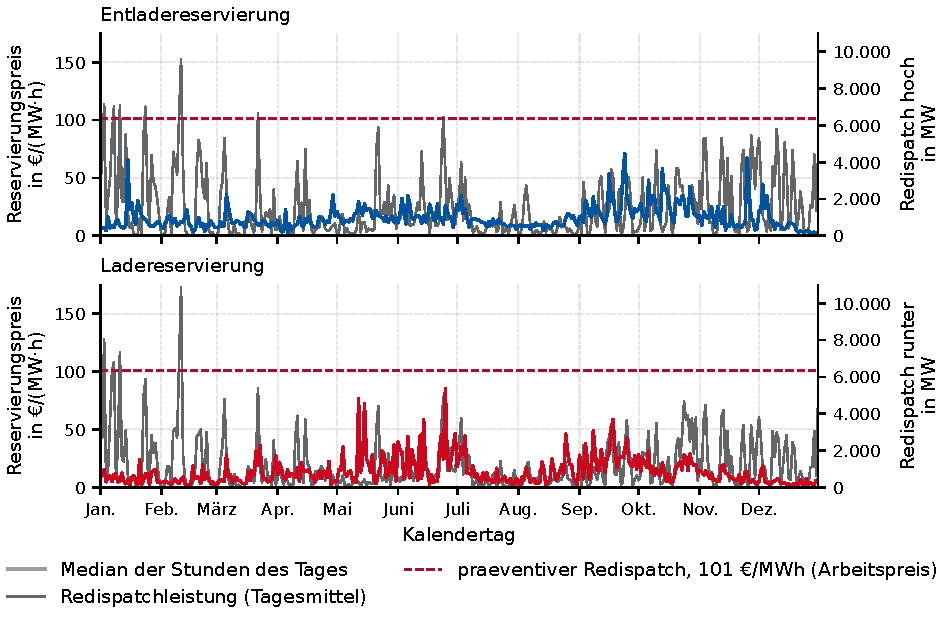
\includegraphics[width=\textwidth]{figures/chapter_4/jahreslauf_reservierungspreis_redispatch_2025_median.pdf}
    \caption{Median des kurativen Reservierungspreises je Tag des Jahres 2025 neben der Redispatchleistung im Tagesmittel, oben entladend und unten ladend.}
    \label{fig:jahreslauf_median}
\end{figure}
